\chapter{Faktor Boltzmann}\label{ch:b2:boltzmann-factor}

Dakilah sebuah gunung dan udaranya menipis: pada tiga ribu meter
tekanannya telah turun menjadi \qty{0.7}{bar}, di puncak Everest menjadi sepertiga
nilai permukaan lautnya. Tak ada yang mengurung atmosfernya dari atas; ia
ditahan gravitasi lalu disebarkan keriuhan termal, dan
kompromi antara keduanya adalah sebuah eksponensial, $n \propto
\eu^{-mgz/k_BT}$ --- nisbah energi potensial sebuah molekul terhadap
$k_BT$ memutuskan seberapa jarang ia di sana atas. Eksponensial yang sama mengatur
bagian atom dalam sebuah aras tereksitasi, jumlah molekul yang cukup cepat
untuk melepaskan diri dari sebuah planet, magnetisasi sebuah paramagnet,
populasi yang harus dibalikkan sebuah laser, dan kuantum yang dicacah hukum
Planck: itulah \emph{faktor Boltzmann}, satu rumus yang paling berguna
dalam fisika statistik. Bab ini memotivasinya dengan
atmosfernya, menyatakannya secara umum, lalu menarik darinya, hanya dengan
jumlah dan integral Gauss, sistem dua aras dan kapasitas
kalornya, ekuipartisi energinya, sebaran kelajuan molekulnya,
dan \omterm{prop:b2:boltzmann-factor:curie}{hukum Curie} paramagnetisme --- dengan, di jalannya, energi rerata
sebuah osilator kuantum, yang merupakan rumus Planck.

\begin{omfigure}
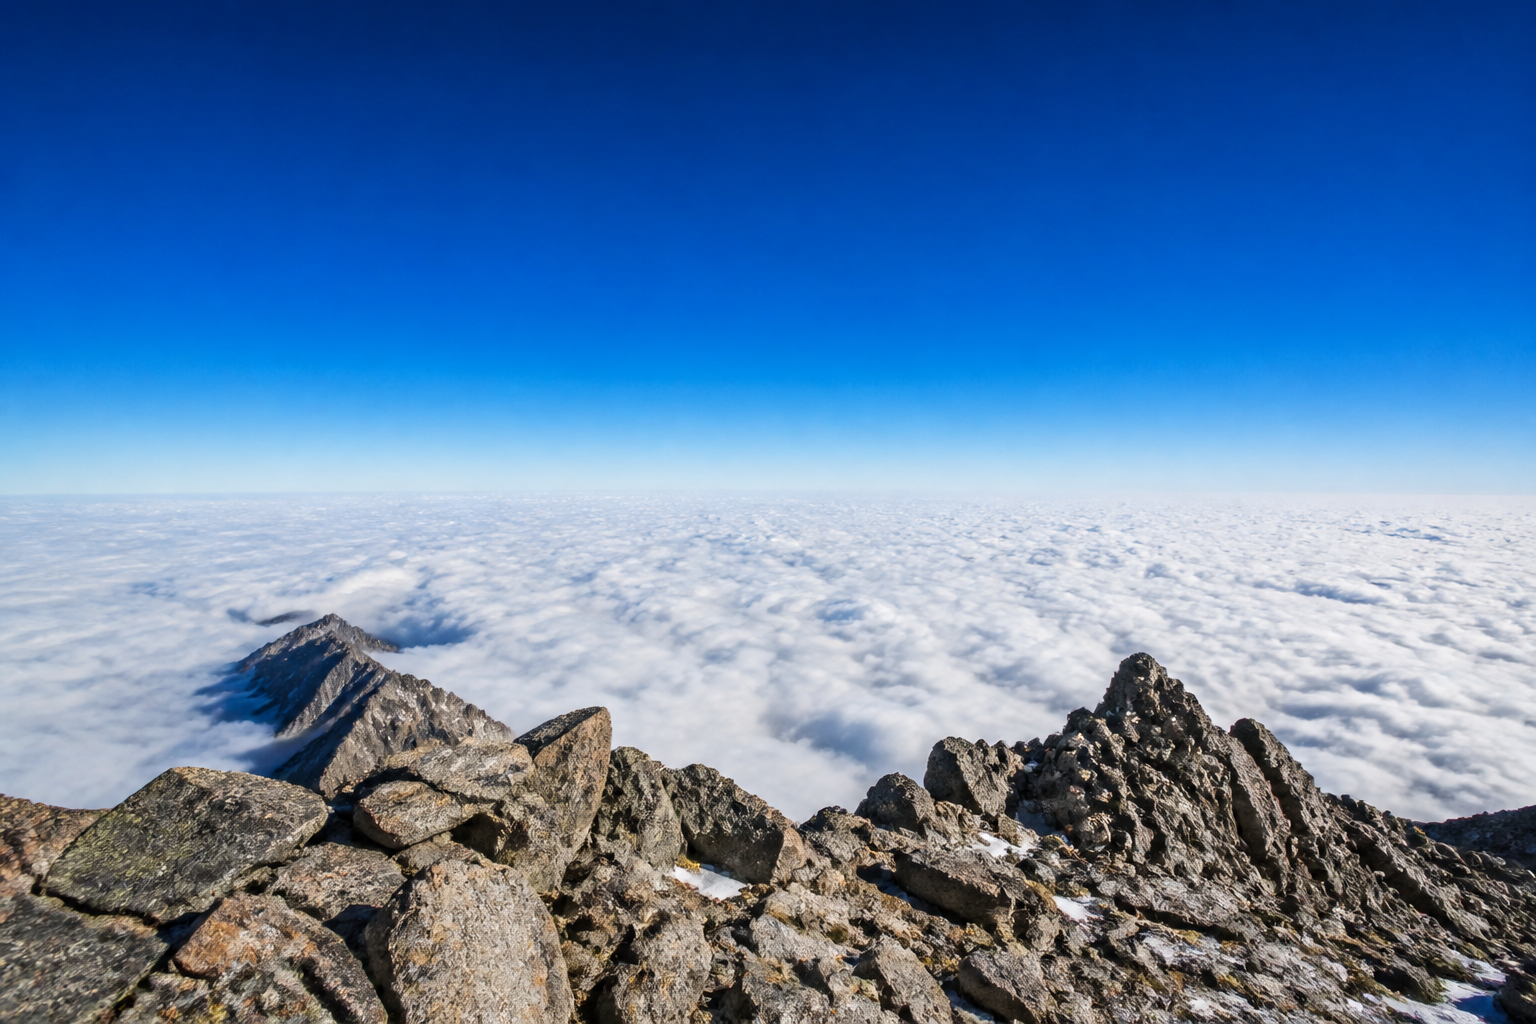
\includegraphics[width=0.58\linewidth]{images/book4/ai/b4-29-sky-gradient-summit.png}

{\small Dari sebuah puncak, kabut atmosfer bawahnya dan biru pekat
di atasnya: kerapatan udaranya turun sebesar faktor $\eu$ tiap
\qty{8}{km} --- yaitu faktor Boltzmann energi potensial sebuah molekul dalam
gravitasi Bumi.}
\end{omfigure}

\section{Atmosfer isotermal}

\begin{proposition}[Hukum barometrik]\label{prop:b2:boltzmann-factor:barometric}
Dalam sebuah atmosfer gas sempurna (bermassa molekul $m$) pada suhu
seragam $T$ dalam gravitasi seragam $g$, tekanan dan \omterm{def:b2:particle-diffusion:flux}{rapat
cacahnya} turun eksponensial dengan ketinggiannya:
\[
P(z) = P_0\,\eu^{-z/H}, \qquad n(z) = n_0\,\eu^{-mgz/k_BT}, \qquad
H = \frac{k_BT}{mg} ,
\]
dengan \emph{tinggi skala}\index{tinggi skala} $H \approx \qty{8.4}{km}$
bagi udara pada \qty{288}{K}. Eksponennya adalah nisbah energi
potensial $mgz$ sebuah molekul terhadap energi termalnya $k_BT$.
\end{proposition}

\begin{proof}
Hidrostatika, $\dd P/\dd z = -\rho g = -nmg$, dan hukum gas sempurnanya $P
= nk_BT$: $\dd P/\dd z = -(mg/k_BT)P$, sebuah eksponensial. Atmosfer
yang sungguhan mendingin dengan ketinggiannya (sekitar \qty{6.5}{K/km} dalam sepuluh
kilometer terbawahnya), yang membuat penurunannya agak lebih cepat; model
isotermalnya baik sampai $20\%$.
\end{proof}

\begin{omfigure}
\begin{tikzpicture}
  \begin{axis}[omaxis, width=8.2cm, height=4.8cm, xmin=0, xmax=32, ymin=0, ymax=1.1,
    xlabel={$z$ (\unit{km})}, ylabel={$P/P_0$}, xtick={8.4,16.8,25.2}, xticklabels={$H$,$2H$,$3H$}, ytick={0.37,1}, yticklabels={$1/\eu$,$1$}, clip=false,
    legend style={font=\scriptsize, at={(0.97,0.45)}, anchor=north east, draw=none, fill=none}]
    \addplot[omDef, thick, domain=0:32, samples=80] {exp(-x/8.4)};
    \addlegendentry{udara, \qty{288}{K}}
    \addplot[omExo, thick, dashed, domain=0:32, samples=80] {exp(-x/60)};
    \addlegendentry{helium saja, $H = \qty{60}{km}$}
    \draw[dashed, gray] (axis cs:8.4,0) -- (axis cs:8.4,0.37) -- (axis cs:0,0.37);
  \end{axis}
\end{tikzpicture}

{\small Atmosfer isotermalnya: tekanan dan kerapatannya turun sebesar $1/\eu$
tiap \omterm{prop:b2:boltzmann-factor:barometric}{tinggi skala} $H = k_BT/mg$; sebuah gas yang lebih ringan akan mempunyai $H$ yang lebih besar
--- tetapi di bawah \qty{100}{km} pergolakan menjaga udaranya tercampur, dan semua
gasnya berbagi $H$ reratanya.}
\end{omfigure}

\section{Faktor Boltzmann}

\begin{theorem}[Faktor Boltzmann]\label{thm:b2:boltzmann-factor:factor}
Sebuah sistem dalam kesetimbangan termal dengan sebuah termostat pada suhu
$T$ ditemukan dalam sebuah keadaan mikroskopis tertentu berenergi $E$ dengan
peluang yang sebanding dengan
\[
\eu^{-E/k_BT} .
\]
Maka, bagi sehimpunan keadaan diskret berenergi $E_i$,
\[
p_i = \frac{\eu^{-E_i/k_BT}}{Z}, \qquad Z = \sum_i\eu^{-E_i/k_BT} ,
\]
dengan jumlah $Z$ (yaitu \emph{fungsi partisi}\index{fungsi partisi})
menormalkan peluangnya; dua keadaan (atau dua aras berdegenerasi
sama) terisi dengan nisbah $N_2/N_1 = \eu^{-(E_2 - E_1)/k_BT}$;
dan bagi sebuah peubah sinambung (sebuah kedudukan, sebuah kecepatan) rapat
peluangnya sebanding dengan $\eu^{-E/k_BT}$ dalam peubah itu. Pada
\qty{300}{K}, $k_BT = \qty{4.1e-21}{J} = \qty{0.026}{eV}$: apa pun yang
memakan jauh lebih banyak daripada ini itu jarang, apa pun yang memakan jauh lebih sedikit
tereksitasi dengan bebas.
\end{theorem}

\begin{proof}
Hukum barometriknya adalah faktornya bagi energi potensial $mgz$; kita
menerima keumumannya, tetapi inilah alasannya (yang diketatkan dalam
jilid Tahun 3). Termostatnya $R$ besar; ketika sistem kecil kita berada dalam
sebuah keadaan berenergi $E$, termostatnya berenergi $E_{\text{tot}} -
E$, dan dapat berada dalam $\Omega_R(E_{\text{tot}} - E)$ keadaan mikroskopis, yang semuanya
sama mungkin (yaitu postulat dasar bagi sebuah keseluruhan yang terkucil). Jadi
$p(E) \propto \Omega_R(E_{\text{tot}} - E)$. Dengan definisi Boltzmann
tentang entropinya, $S_R = k_B\ln\Omega_R$, dan $1/T = \dd S_R/\dd E_R$ bagi
termostatnya, $\ln\Omega_R(E_{\text{tot}} - E) \approx \ln\Omega_R(E_{\text{tot}})
- E/k_BT$ karena $E \ll E_{\text{tot}}$; eksponenkanlah.
\end{proof}

\begin{example}[Populasi aras atomik]\label{ex:b2:boltzmann-factor:levels}
Aras tereksitasi pertama hidrogen terletak \qty{10.2}{eV} di atas keadaan
dasarnya: pada \qty{300}{K}, $\eu^{-395}$ --- tak satu atom pun di alam semesta; pada
\qty{6000}{K}, yaitu permukaan Matahari, $\eu^{-19.7} \approx 3 \times 10^{-9}$ (dikalikan
degenerasi $4$): cukup, dalam kolom gas Matahari yang besar, bagi
garis serapan Balmernya, yang terkuat pada bintang dekat \qty{10000}{K}.
Garis D natrium (\qty{2.1}{eV}) dalam sebuah nyala \qty{2500}{K}: $\eu^{-9.8} = 6
\times 10^{-5}$ atomnya tereksitasi, yang memberi nyala kuning sejumput
garam. Dan medium laser \cref{ch:b2:laser}: faktornya
mengatakan bahwa aras atasnya kosong pada kesetimbangan, dan pompanya harus melawan
faktor itu.
\end{example}

\section{Aras diskret: sistem dua aras dan osilatornya}

\begin{proposition}[Energi rerata dari fungsi partisinya]\label{prop:b2:boltzmann-factor:meanE}
Dengan $\beta = 1/k_BT$,
\[
\langle E\rangle = \sum_ip_iE_i = -\frac{\partial\ln Z}{\partial\beta}, \qquad
C = \frac{\dd\langle E\rangle}{\dd T} .
\]
\end{proposition}

\begin{proof}
$\partial_\beta Z = -\sum E_i\eu^{-\beta E_i}$, bagilah dengan $Z$.
\end{proof}

\begin{proposition}[Sistem dua aras]\label{prop:b2:boltzmann-factor:twolevel}
$N$ sistem yang saling bebas dengan dua aras $0$ dan $\varepsilon$ (spin dalam sebuah
medan, atom dengan satu aras tereksitasi, cacat dengan dua kedudukan):
\[
\frac{N_2}{N} = \frac{1}{\eu^{\varepsilon/k_BT} + 1}, \qquad
\langle E\rangle = \frac{N\varepsilon}{\eu^{\varepsilon/k_BT} + 1}, \qquad
C = Nk_B\,\frac{x^2\eu^x}{(\eu^x + 1)^2}, \quad x = \frac{\varepsilon}{k_BT} .
\]
Aras atasnya kosong pada suhu rendah dan paling banter terisi separuh pada
suhu tinggi (tak pernah terbalik pada kesetimbangan); kapasitas kalornya
lenyap di kedua ujungnya lalu memuncak pada $0.44\,Nk_B$ dekat $k_BT = 0.42
\varepsilon$ --- yaitu \emph{anomali Schottky}\index{anomali Schottky}, yaitu
tanda sebuah senjang dalam spektrumnya.
\end{proposition}

\begin{proof}
$Z = 1 + \eu^{-x}$; $p_2 = \eu^{-x}/(1 + \eu^{-x})$; turunkanlah $\langle
E\rangle$ terhadap $T$.
\end{proof}

\begin{omfigure}
\begin{tikzpicture}
  \begin{axis}[omaxis, width=6.4cm, height=4.4cm, xmin=0, xmax=3.2, ymin=0, ymax=1.1,
    xlabel={$k_BT/\varepsilon$}, ylabel={populasi}, xtick={1,2,3}, ytick={0.5,1}, clip=false]
    \addplot[omDef, thick, domain=0.02:3.2, samples=100] {1/(exp(1/x)+1)};
    \addplot[omExo, thick, domain=0.02:3.2, samples=100] {exp(1/x)/(exp(1/x)+1)};
    \node[font=\scriptsize, omExo] at (axis cs:1.4,0.85) {$N_1/N$};
    \node[font=\scriptsize, omDef] at (axis cs:1.4,0.2) {$N_2/N$};
  \end{axis}
  \begin{axis}[omaxis, width=6.4cm, height=4.4cm, xmin=0, xmax=3.2, ymin=0, ymax=0.55, xshift=6.6cm,
    xlabel={$k_BT/\varepsilon$}, ylabel={$C/Nk_B$}, xtick={1,2,3}, ytick={0.44}, clip=false]
    \addplot[omThm, thick, domain=0.08:3.2, samples=120] {(1/x)^2*exp(1/x)/(exp(1/x)+1)^2};
    \draw[dashed, gray] (axis cs:0.42,0) -- (axis cs:0.42,0.44);
    \node[font=\scriptsize, below] at (axis cs:0.42,0) {$0.42$};
  \end{axis}
\end{tikzpicture}

{\small Sistem dua arasnya: populasinya terhadap suhu (aras
atasnya terisi menuju setengah, tak pernah lebih) dan kapasitas kalor
Schottkynya, sebuah bonggol di tempat $k_BT$ sepadan dengan senjangnya.}
\end{omfigure}

\begin{proposition}[Osilator kuantum dan rumus Planck]\label{prop:b2:boltzmann-factor:oscillator}
Sebuah osilator selaras berfrekuensi $\nu$ mempunyai aras $E_n = nh\nu$ (ditambah
sebuah tetapan); pada suhu $T$,
\[
Z = \frac{1}{1 - \eu^{-h\nu/k_BT}}, \qquad
\langle E\rangle = \frac{h\nu}{\eu^{h\nu/k_BT} - 1}
\ \longrightarrow\
\begin{cases} k_BT & (h\nu \ll k_BT), \\ h\nu\,\eu^{-h\nu/k_BT} & (h\nu \gg k_BT). \end{cases}
\]
Inilah energi rerata sebuah ragam medan radiasi yang dikalikan hukum
Planck (\cref{ch:b2:thermal-radiation}) dengan jumlah ragamnya,
dan energi rerata sebuah getaran dalam sebuah zat padat: pada suhu tinggi
$k_BT$ klasiknya, pada suhu rendah sebuah ragam yang beku.
\end{proposition}

\begin{proof}
Deret ukur, lalu $-\partial_\beta\ln Z$.
\end{proof}

\begin{example}[Kapasitas kalor zat padat]\label{ex:b2:boltzmann-factor:einstein}
Perlakukanlah tiap atom sebuah zat padat sebagai tiga osilator berfrekuensi sama
$\nu$ (Einstein, 1907): $C = 3Nk_B\,x^2\eu^x/(\eu^x - 1)^2$ dengan $x =
h\nu/k_BT$. Di atas $\theta_{\text{E}} = h\nu/k_B$, $C \to 3Nk_B = 3R$ tiap mol
--- yaitu hukum Dulong dan Petit (\qty{25}{J/mol/K}), yang dituruti timbal,
tembaga, besi pada suhu ruang; jauh di bawahnya, $C$ runtuh. Intan
($\theta_{\text{E}} \approx \qty{1300}{K}$) hanya mempunyai \qty{6}{J/mol/K} pada
\qty{300}{K}, yang tak dapat dijelaskan fisika klasik, dan kapasitas kalor setiap
zat padat lenyap pada suhu rendah --- yaitu keberhasilan pertama
kuantum di luar radiasinya.
\end{example}

\section{Ekuipartisi dan sebaran Maxwell}

\begin{theorem}[Ekuipartisi energi]\label{thm:b2:boltzmann-factor:equipartition}
Setiap peubah $q$ yang masuk ke energinya secara kuadratik, $E = aq^2 +
\dots$, dan berjangkau seluruh nilai nyata, menyumbang $\tfrac12k_BT$ pada
energi rerata pada kesetimbangannya:
\[
\langle aq^2\rangle = \tfrac12k_BT .
\]
Sebuah gas monoatomik (tiga translasi) mempunyai $U = \tfrac32Nk_BT$ dan $C_V =
\tfrac32R$ tiap mol; sebuah gas diatomik menambahkan dua rotasi, $C_V = \tfrac52R$,
dan getarannya (dua suku kuadratik, tetapi terkuantumkan dengan $h\nu \gg
k_BT$ pada suhu ruang) tetap beku sampai beberapa ribu kelvin.
\end{theorem}

\begin{proof}
Rapat peluangnya dalam $q$ adalah $\propto\eu^{-aq^2/k_BT}$, sebuah Gauss:
\[
\langle aq^2\rangle = \frac{\int aq^2\,\eu^{-aq^2/k_BT}\,\dd q}{\int\eu^{-aq^2/k_BT}\,\dd q} = \tfrac12k_BT
\]
(turunkanlah $\int\eu^{-\lambda q^2}\dd q = \sqrt{\pi/\lambda}$ terhadap
$\lambda$). Hasilnya menuntut kesinambungannya: ketika
arasnya berjarak lebih daripada $k_BT$ faktornya membekukan peubahnya,
seperti bagi osilator di atas.
\end{proof}

\begin{theorem}[Sebaran kelajuan Maxwell]\label{thm:b2:boltzmann-factor:maxwell}
Dalam sebuah gas pada $T$, komponen kecepatannya adalah Gauss yang saling bebas bervariansi
$k_BT/m$, dan kelajuannya $v = |\vect v|$ mempunyai rapat
peluang
\[
f(v) = 4\pi\Big(\frac{m}{2\pi k_BT}\Big)^{3/2}v^2\,\eu^{-mv^2/2k_BT} ,
\]
dengan kelajuan paling mungkin, rerata dan akar kuadrat reratanya
\[
v_{\text{p}} = \sqrt{\frac{2k_BT}{m}}, \qquad
\langle v\rangle = \sqrt{\frac{8k_BT}{\pi m}}, \qquad
v_{\text{rms}} = \sqrt{\frac{3k_BT}{m}} ,
\]
dengan nisbah $1 : 1.13 : 1.22$. Bagi nitrogen pada \qty{300}{K}: \qty{422}{},
\qty{476}{}, \qty{517}{m/s}; bagi hidrogen, $3.7$ kali lebih banyak;
ekor sebarannya, $\propto\eu^{-mv^2/2k_BT}$, adalah yang meloloskan
molekul tercepatnya menguap, bereaksi, atau meninggalkan sebuah planet.
\end{theorem}

\begin{proof}
Energi kinetiknya $\tfrac12m(v_x^2 + v_y^2 + v_z^2)$ memberi faktor
$\eu^{-mv_x^2/2k_BT}\eu^{-mv_y^2/2k_BT}\eu^{-mv_z^2/2k_BT}$: yaitu tiga Gauss yang saling
bebas, masing-masingnya dinormalkan oleh $\sqrt{m/2\pi k_BT}$. Sebaran
kelajuannya memungut semua kecepatan dalam selubung berjari-jari $v$ dan
bervolume $4\pi v^2\dd v$. Lalu $v_{\text{p}}$ dari $\dd f/\dd v = 0$, dan
momennya dari $\int_0^\infty v^3\eu^{-av^2}\dd v = 1/2a^2$, $\int_0^\infty
v^4\eu^{-av^2}\dd v = \tfrac38\sqrt{\pi/a^5}$; $v_{\text{rms}}$ juga menyusul
dari ekuipartisinya, $\tfrac12m\langle v^2\rangle = \tfrac32k_BT$.
\end{proof}

\begin{omfigure}
\begin{tikzpicture}
  \begin{axis}[omaxis, width=9cm, height=5cm, xmin=0, xmax=1750, ymin=0, ymax=0.0028,
    xlabel={$v$ (\unit{m/s})}, ylabel={$f(v)$}, xtick={400,800,1200}, ytick=\empty, clip=false,
    legend style={font=\scriptsize, at={(0.97,0.95)}, anchor=north east, draw=none, fill=none}]
    \addplot[omDef, thick, domain=0:1600, samples=160] {4*pi*(28*1.66e-27/(2*pi*1.38e-23*100))^1.5*x^2*exp(-28*1.66e-27*x^2/(2*1.38e-23*100))};
    \addlegendentry{N$_2$, \qty{100}{K}}
    \addplot[omThm, thick, domain=0:1600, samples=160] {4*pi*(28*1.66e-27/(2*pi*1.38e-23*300))^1.5*x^2*exp(-28*1.66e-27*x^2/(2*1.38e-23*300))};
    \addlegendentry{N$_2$, \qty{300}{K}}
    \addplot[omExo, thick, domain=0:1600, samples=160] {4*pi*(28*1.66e-27/(2*pi*1.38e-23*1000))^1.5*x^2*exp(-28*1.66e-27*x^2/(2*1.38e-23*1000))};
    \addlegendentry{N$_2$, \qty{1000}{K}}
  \end{axis}
\end{tikzpicture}

{\small Sebaran kelajuan Maxwell bagi nitrogen pada tiga
suhu: puncaknya beranjak sebagai $\sqrt T$, kurvanya melebar, dan
ekor berkelajuan tingginya tumbuh tercepat dari semuanya --- yaitu ekor yang memutuskan pelepasan
dan laju reaksinya.}
\end{omfigure}

\begin{example}[Siapa yang meninggalkan planetnya]\label{ex:b2:boltzmann-factor:escape}
Kelajuan lepas Bumi adalah \qty{11.2}{km/s}. Dalam eksosfernya, dekat
\qty{1000}{K}, helium mempunyai $v_{\text{p}} = \qty{2.0}{km/s}$: bagian
atom di atas kelajuan lepasnya berorde $\eu^{-(11.2/2.0)^2} = \eu^{-31}
\approx 10^{-13}$ --- kecil, tetapi diperbarui pada tiap tumbukan selama bermiliar
tahun: helium merembes pergi, dan kelimpahannya dalam udara hanya
\qty{5}{ppm} meskipun produksinya tetap lewat peluruhan radioaktif. Bagi
nitrogen eksponennya tujuh kali lebih besar, $\eu^{-220}$: nitrogen tinggal.
Di Bulan ($v_{\text{lepas}} = \qty{2.4}{km/s}$) bahkan nitrogen pada
\qty{400}{K} ($v_{\text{p}} = \qty{490}{m/s}$) mempunyai $\eu^{-24}$ tiap waktu tumbukan:
sepanjang umur tata suryanya, tak ada atmosfer yang bertahan.
\end{example}

\section{Paramagnetisme dan hukum Curie}

\begin{proposition}[Paramagnet spin 1/2]\label{prop:b2:boltzmann-factor:curie}
$N$ momen magnet yang saling bebas yang hanya dapat menunjuk searah atau berlawanan dengan
medannya $B$, berenergi $\mp\mu B$, mempunyai pada suhu $T$ momen dan
magnetisasi rerata
\[
\langle\mu_z\rangle = \mu\tanh\frac{\mu B}{k_BT}, \qquad
M = n\mu\tanh\frac{\mu B}{k_BT}
\ \longrightarrow\
\begin{cases} n\mu^2B/k_BT & (\mu B \ll k_BT):\ \text{hukum Curie}, \\ n\mu & (\mu B \gg k_BT):\ \text{kejenuhan}. \end{cases}
\]
Suseptibilitasnya $\chi = \mu_0M/B = \mu_0n\mu^2/k_BT$ berubah sebagai $1/T$
(\emph{hukum Curie}\index{hukum Curie}); dengan $\mu = \mu_B = \qty{9.27e-24}{J/T}$,
$\mu B/k_BT = 2.2 \times 10^{-3}$ pada \qty{1}{T} dan \qty{300}{K}, sehingga
paramagnet biasa nyaris tak termagnetkan; pada \qty{1}{K} medan yang sama memberi
$0.67$ dan kejenuhannya mulai.
\end{proposition}

\begin{proof}
$p_\pm \propto\eu^{\pm\mu B/k_BT}$: $\langle\mu_z\rangle = \mu(\eu^x - \eu^{-x})/(\eu^x +
\eu^{-x})$ dengan $x = \mu B/k_BT$; $\tanh x \approx x$ bagi $x$ yang kecil.
\end{proof}

\begin{omfigure}
\begin{tikzpicture}
  \begin{axis}[omaxis, width=8.2cm, height=4.6cm, xmin=0, xmax=3.2, ymin=0, ymax=1.15,
    xlabel={$x = \mu B/k_BT$}, ylabel={$M/n\mu$}, xtick={1,2,3}, ytick={1}, clip=false]
    \addplot[omDef, thick, domain=0:3.2, samples=100] {tanh(x)};
    \addplot[omExo, dashed, domain=0:1.1] {x};
    \node[font=\scriptsize, omExo, anchor=west] at (axis cs:1.1,1.08) {Curie: $M \propto B/T$};
    \node[font=\scriptsize, omDef, anchor=west] at (axis cs:2.0,0.88) {kejenuhan};
  \end{axis}
\end{tikzpicture}

{\small Magnetisasi sebuah paramagnet spin 1/2: linear dalam $B/T$ pada
medan kecil (Curie), menjenuh ketika $\mu B$ melampaui $k_BT$ --- yang dicapai
pada satu tesla hanya di bawah satu kelvin, yang membuat kurvanya sebuah termometer
bagi percobaan yang terdingin.}
\end{omfigure}

\begin{remark}[Apa yang tak dilakukan faktornya]\label{rem:b2:boltzmann-factor:limits}
Faktor Boltzmann melukiskan \emph{kesetimbangan} pada sebuah suhu; ia
tak mengatakan apa pun tentang laju (seberapa cepat kesetimbangannya tercapai --- meskipun
sebuah energi aktivasi $E_{\text{a}}$ memberi laju $\propto\eu^{-E_{\text{a}}/k_BT}$,
yaitu hukum Arrhenius yang dijumpai bagi difusi dalam zat padat). Ia berlaku bagi
subsistem yang saling bebas atau bagi keseluruhannya; bagi partikel kuantum yang
serupa pada kerapatan tinggi (elektron dalam sebuah logam, foton, helium dekat
nol mutlak) ia digantikan sebaran Fermi--Dirac dan Bose--Einstein
jilid Tahun 3, yang ia merupakan limit encernya.
\end{remark}

\begin{method}[Taksiran Boltzmann]\label{meth:b2:boltzmann-factor:method}
(1) Hitunglah $E/k_BT$; $k_BT = \qty{0.026}{eV}$ pada \qty{300}{K}, \qty{1}{eV}
pada \qty{11600}{K}. (2) Nisbah populasinya: $\eu^{-\Delta E/k_BT}$ (dikalikan
degenerasinya). (3) Aras diskret: $Z$, lalu $\langle E\rangle =
-\partial_\beta\ln Z$, lalu $C$. (4) Peubah sinambung yang kuadratik:
$\tfrac12k_BT$ masing-masingnya, jika tak beku. (5) Kelajuan: $v_{\text{p}} = \sqrt{2k_BT/m}$
dan ekor Gaussnya. (6) Spin: $\tanh(\mu B/k_BT)$, $1/T$ Curienya.
\end{method}

\section{Latihan}

\begin{exercise}[$\star$]\label{exo:b2:boltzmann-factor:1}
Tentukanlah \omterm{prop:b2:boltzmann-factor:barometric}{tinggi skala} udara pada \qty{288}{K} ($M = \qty{29}{g/mol}$); tekanannya pada
\qty{3000}{m}, pada \qty{8849}{m}, pada \qty{10}{km} (bandingkanlah dengan \qty{0.26}{bar}
yang terukur); \omterm{prop:b2:boltzmann-factor:barometric}{tinggi skala} helium saja; dan \omterm{prop:b2:boltzmann-factor:barometric}{tinggi skala} atmosfer Mars
(CO$_2$, \qty{210}{K}, $g = \qty{3.7}{m/s^2}$).
\end{exercise}

\begin{exercise}[$\star$]\label{exo:b2:boltzmann-factor:2}
Populasi: aras $n = 2$ hidrogen (\qty{10.2}{eV}, degenerasinya $4$
melawan $1$) pada \qty{300}{K}, \qty{6000}{K}, \qty{10000}{K}; aras
\qty{2.1}{eV} natrium dalam sebuah nyala \qty{2500}{K}; sebuah aras rotasi molekul pada
\qty{1e-3}{eV} pada \qty{300}{K}; sebuah aras spin inti yang terbelah sebesar \qty{1e-7}{eV} dalam
sebuah magnet pada \qty{300}{K}.
\end{exercise}

\begin{exercise}[$\star$]\label{exo:b2:boltzmann-factor:3}
Tentukanlah kelajuan Maxwell ($v_{\text{p}}$, $\langle v\rangle$, $v_{\text{rms}}$) bagi N$_2$
pada \qty{300}{K} dan \qty{77}{K}, H$_2$ pada \qty{300}{K}, dan bagi sebutir asap
bermassa \qty{1e-18}{kg}. Berapa bagian molekul yang lebih cepat daripada $2v_{\text{p}}$
(sekitar $4.6\%$) dan daripada $3v_{\text{p}}$ (sekitar $4 \times 10^{-4}$): ulaslah
ekornya.
\end{exercise}

\begin{exercise}[$\star$]\label{exo:b2:boltzmann-factor:4}
Momen spin 1/2 ber-$\mu = \mu_B$, $n = \qty{1e28}{m^{-3}}$, $B = \qty{1}{T}$:
tentukanlah $x = \mu B/k_BT$ pada \qty{300}{K} dan \qty{1}{K}; $M/M_{\text{jenuh}}$; $M_{\text{jenuh}}$;
suseptibilitasnya pada \qty{300}{K}. Bandingkanlah dengan magnetisasi jenuh
besi (\qty{1.7e6}{A/m}).
\end{exercise}

\begin{exercise}[$\star\star$]\label{exo:b2:boltzmann-factor:5}
\emph{Dua aras.} (a) Turunkanlah $p_1$, $p_2$, $\langle E\rangle$ dari $Z$. (b)
Tunjukkanlah bahwa $N_2 < N_1$ pada setiap suhu positif; apa artinya $N_2 >
N_1$ bagi $T$? (c) Tentukanlah entropi $S = -Nk_B\sum p_i\ln p_i$ sistemnya pada
$T \to 0$ dan $T \to \infty$. (d) Sebuah cacat dalam sebuah hablur dapat duduk dalam dua
kedudukan yang terpisah \qty{0.05}{eV}: berapa penghunian kedudukan atasnya pada
\qty{300}{K} dan pada \qty{77}{K}.
\end{exercise}

\begin{exercise}[$\star\star$]\label{exo:b2:boltzmann-factor:6}
\emph{Schottky.} (a) Turunkanlah $C(T)$ sistem dua arasnya. (b) Tempatkanlah
maksimumnya secara numerik ($x = 2.40$) dan nilainya. (c) Limitnya pada $T$ rendah
dan tinggi, dengan makna fisisnya. (d) Spin inti tembaga
dalam \qty{1}{T} mempunyai $\varepsilon \approx \qty{1e-7}{eV}$: pada suhu berapa
puncak Schottkynya duduk, dan mengapa ia berarti bagi kriostat
yang terdingin?
\end{exercise}

\begin{exercise}[$\star\star$]\label{exo:b2:boltzmann-factor:7}
\emph{Ekuipartisi dan kegagalannya.} (a) Turunkanlah $\langle aq^2\rangle =
k_BT/2$ dengan integral Gaussnya. (b) Tentukanlah $C_V$ sebuah gas monoatomik dan sebuah
gas diatomik yang tegar. (c) Getaran nitrogen mempunyai $h\nu/k_B = \qty{3400}{K}$:
dengan memakai energi rerata osilatornya, tentukanlah $C_V$ pada \qty{300}{K}, \qty{1000}{K},
\qty{3000}{K}. (d) Zat padat Einstein: tentukanlah $C$ pada $T = \theta_{\text{E}}$, $\theta_{\text{E}}/4$,
$4\theta_{\text{E}}$ dalam satuan $3R$; dan intan pada suhu ruang.
\end{exercise}

\begin{exercise}[$\star\star$]\label{exo:b2:boltzmann-factor:8}
\emph{Maxwell secara rinci.} (a) Tunjukkanlah bahwa komponen kecepatannya adalah
Gauss yang saling bebas lalu turunkanlah $f(v)$. (b) Hitunglah $v_{\text{p}}$,
$\langle v\rangle$, $v_{\text{rms}}$. (c) Energi kinetik reratanya: periksalah dengan
ekuipartisinya. (d) Fluks molekul yang menumbuk sebuah dinding adalah
$\tfrac14n\langle v\rangle$ tiap satuan luas dan waktu (diterima tanpa bukti): berapa jumlah
molekul N$_2$ yang menumbuk \qty{1}{cm^2} tiap sekon pada \qty{1}{bar},
\qty{300}{K}; dan laju sebuah lubang jarum \qty{1}{\micro m} meloloskan udara
ke dalam sebuah kamar hampa (efusi).
\end{exercise}

\begin{exercise}[$\star\star$]\label{exo:b2:boltzmann-factor:9}
\emph{Pelepasan.} (a) Berapa bagian sebuah gas Maxwell yang lebih cepat daripada $v$: tunjukkanlah bahwa ia
kira-kira $(2/\sqrt\pi)\,x\,\eu^{-x^2}$ bagi $x = v/v_{\text{p}} \gg 1$.
(b) Helium pada \qty{1000}{K} di atas \qty{11.2}{km/s}; dan nitrogennya. (c) Bulan,
$v_{\text{lepas}} = \qty{2.4}{km/s}$, \qty{400}{K}: nitrogennya, dan suhu
berapa yang akan menahannya selama umur tata suryanya (ambillah $10^{17}$
waktu tumbukan: bagian yang lepasnya di bawah $10^{-17}$). (d) Mengapa Titan
(\qty{2.6}{km/s}, \qty{94}{K}) menyimpan sebuah atmosfer nitrogen yang tebal?
\end{exercise}

\begin{exercise}[$\star\star\star$]\label{exo:b2:boltzmann-factor:10}
\emph{Potensial lain.} (a) Dalam sebuah sentrifus yang berputar pada $\omega$,
energi potensial efektifnya adalah $-\tfrac12m\omega^2r^2$: tentukanlah profil kerapatannya
$n(r)$. (b) Uranium heksafluorida, dua isotop $\Delta m = \qty{3}{u}$, $\omega
= 2\pi \times \qty{1000}{Hz}$, $r = \qty{10}{cm}$, \qty{300}{K}: berapa faktor
pengayaan satu tingkatnya. (c) Bola koloid (bermassa apung $m' =
\qty{2.6e-17}{kg}$) dalam air pada \qty{293}{K}: berapa \omterm{prop:b2:boltzmann-factor:barometric}{tinggi skala}
kesetimbangan sedimentasinya; bagaimana ini memberi bilangan Avogadro? (d) Sebuah
gas elektron dalam sebuah medan $E$: mengapa profil Boltzmannnya
$\eu^{eEx/k_BT}$ merupakan dasar panjang perisai Debye
$\lambda_{\text{D}} = \sqrt{\varepsilon_0k_BT/ne^2}$ sebuah \omterm{def:b2:waves-in-media:plasma}{plasma} (sketsalah
alasannya)?
\end{exercise}

\begin{exercise}[$\star\star\star$]\label{exo:b2:boltzmann-factor:11}
\emph{Planck dari Boltzmann.} (a) Hitunglah $Z$ dan $\langle E\rangle$ bagi
aras $nh\nu$. (b) Kedua limitnya dan maknanya. (c) Kalikanlah dengan
rapat ragamnya $8\pi\nu^2/c^3$ (diberikan) lalu dapatkanlah kembali hukum Planck;
tunjukkanlah bahwa hukum Rayleigh--Jeans adalah ekuipartisi yang diterapkan pada tiap ragamnya.
(d) Mengapa pencacahan klasiknya gagal, dalam satu kalimat?
\end{exercise}

\begin{exercise}[$\star\star\star$]\label{exo:b2:boltzmann-factor:12}
\emph{Demagnetisasi adiabatik.} Entropi $N$ spin 1/2 adalah $S =
Nk_B[\ln(2\cosh x) - x\tanh x]$, $x = \mu B/k_BT$. (a) Tunjukkanlah bahwa ia hanya bergantung
pada $B/T$, dengan $S \to Nk_B\ln 2$ bagi $B/T \to 0$ dan $S \to 0$ bagi $B/T
\to \infty$. (b) Sebuah garam pada \qty{1}{K} dimagnetkan secara isotermal dari $0$ ke
\qty{1}{T}: berapa entropi yang disingkirkan (tiap spin, dengan $\mu = \mu_B$). (c) Medannya
lalu dikurangi secara adiabatik menjadi \qty{0.01}{T}: berapa suhu akhirnya. (d)
Apa yang membatasi metodenya, dan bagaimana kurva $\tanh$ yang sama melayani sebagai
sebuah termometer?
\end{exercise}

\begin{omfigure}
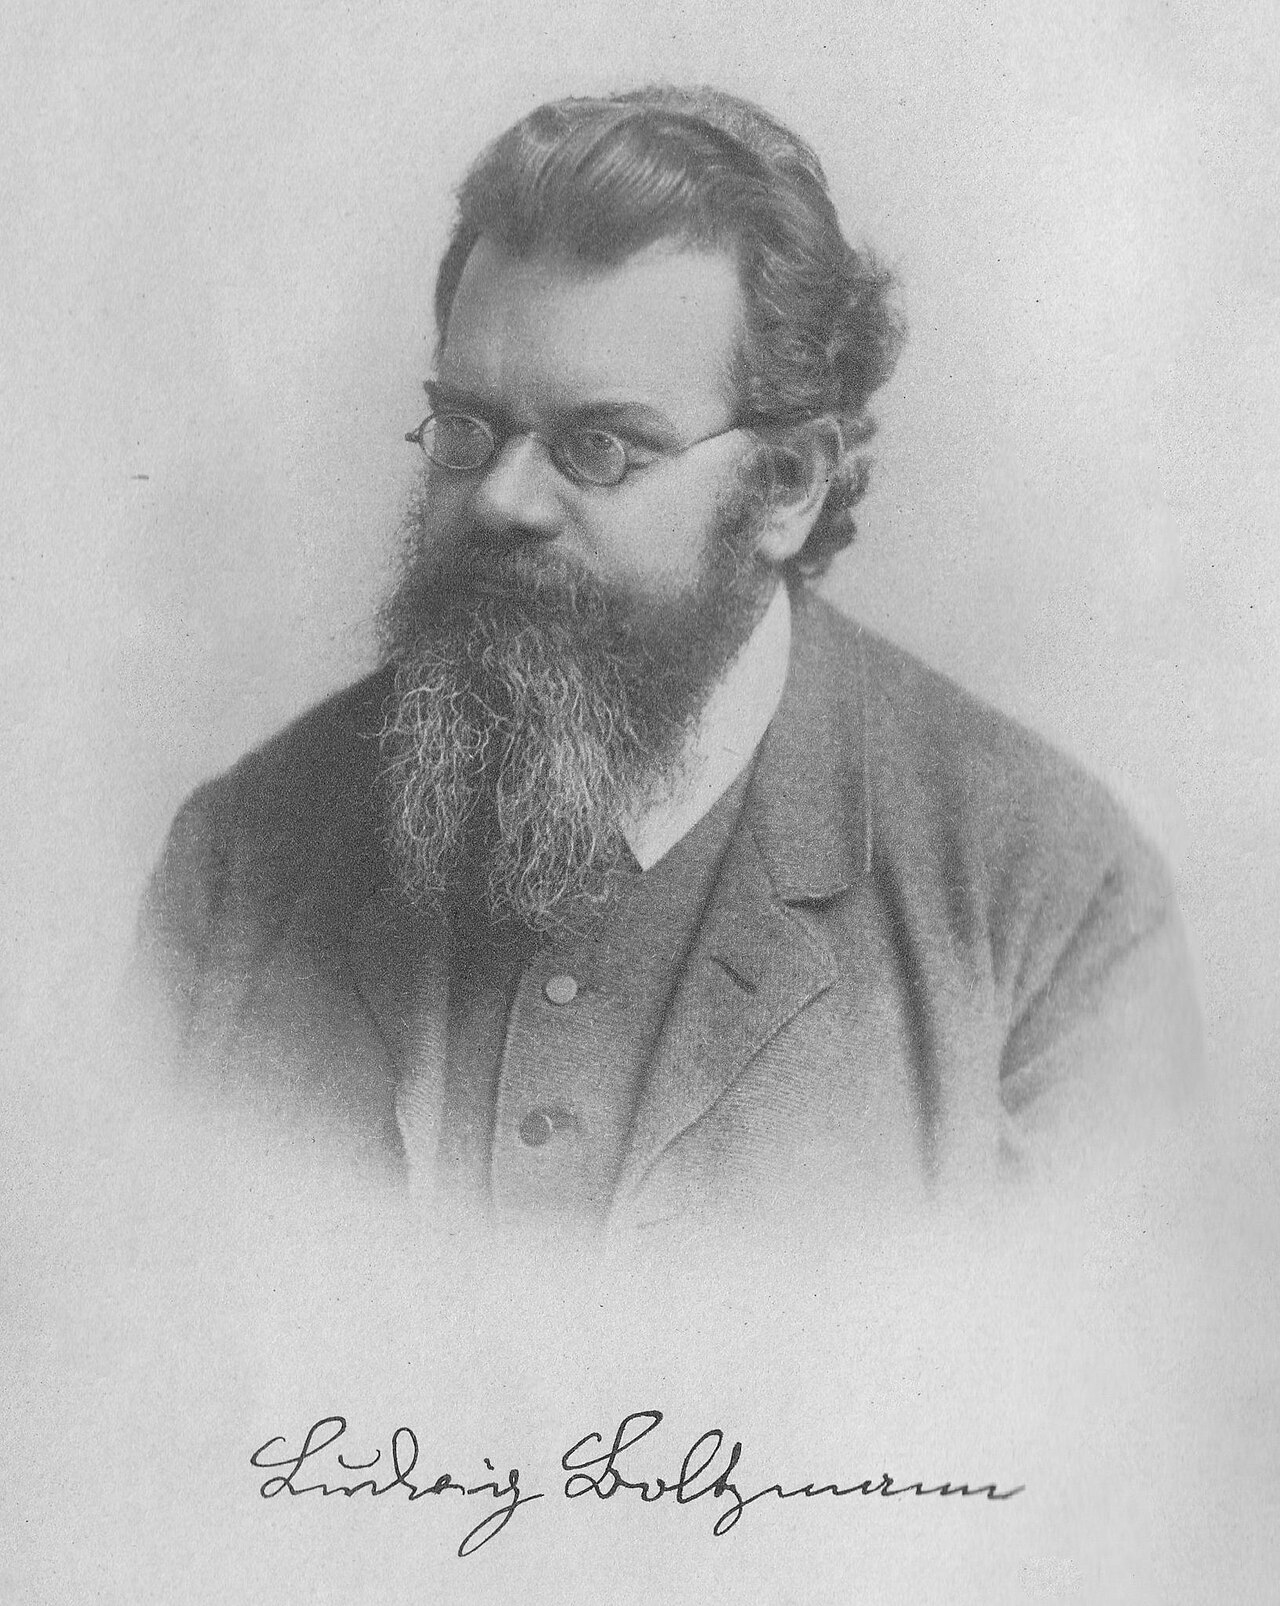
\includegraphics[width=0.3\linewidth]{images/book4/boltzmann-portrait.jpg}

{\small Ludwig Boltzmann (1844--1906), yang faktornya $\eu^{-E/k_BT}$ menjadi pokok bab ini, dan yang rumusnya $S = k_B\ln\Omega$ terukir pada makamnya di Wina.}
\end{omfigure}

\section{Soal: Atmosfer isotermal, lepasnya helium dan sebuah termometer spin}

\begin{problem}[{Soal akhir pekan --- tiga kegunaan satu eksponensial}]\label{pb:b2:boltzmann-factor:1}
Data: $k_B = \qty{1.38e-23}{J/K}$, $N_A = \qty{6.02e23}{mol^{-1}}$, $g =
\qty{9.8}{m/s^2}$, $R_{\oplus} = \qty{6.37e6}{m}$, $\mu_B = \qty{9.27e-24}{J/T}$;
udara $M = \qty{29}{g/mol}$, helium \qty{4}{g/mol}, nitrogen \qty{28}{g/mol}.

\textbf{Bagian I --- Atmosfer isotermalnya.}
\begin{enumerate}
  \item Dari hidrostatika dan hukum gas sempurnanya, turunkanlah $P(z) =
        P_0\eu^{-z/H}$ lalu berikanlah $H$ bagi udara pada \qty{288}{K}.
  \item Kenalilah faktor Boltzmann dalam hasilnya; energi yang mana,
        suhu yang mana?
  \item Tekanannya pada \qty{3000}{m}, \qty{5500}{m} dan \qty{8849}{m};
        ketinggian yang tekanannya menjadi separuh.
  \item Massa atmosfernya tiap meter persegi (dari $P_0 =
        \qty{1.013e5}{Pa}$), dan massa totalnya; periksalah bahwa $\int_0^\infty
        \rho\,\dd z = \rho_0H$.
  \item Jumlah molekul dalam atmosfernya.
  \item Jika tiap gasnya menuruti $H$-nya sendiri, berapa nisbah
        O$_2$/N$_2$ pada \qty{50}{km} dibandingkan dengan di tanahnya? Mengapa
        susunannya sebenarnya seragam sampai \qty{100}{km}?
  \item Troposfer yang sungguhan mendingin sebesar \qty{6.5}{K/km}: lebih tinggi atau lebih rendahkah
        tekanan pada \qty{10}{km} daripada taksiran isotermalnya?
        Jelaskanlah.
  \item \omterm{def:b2:particle-diffusion:flux}{Rapat cacahnya} di permukaan laut dan pada \qty{100}{km} (model
        isotermal, \qty{288}{K}): ulaslah ``tepi antariksa''-nya.
\end{enumerate}

\textbf{Bagian II --- Lepasnya helium.}
Eksosfernya, di atas \qty{500}{km}, berada pada sekitar \qty{1000}{K} dan
tanpa tumbukan: sebuah molekul yang bergerak ke atas lebih cepat daripada kelajuan lepasnya
pergi.
\begin{enumerate}[resume]
  \item Kelajuan lepas dari Bumi pada ketinggian itu.
  \item Kelajuan paling mungkin dan rerata helium dan nitrogen pada
        \qty{1000}{K}.
  \item Berapa bagian atom helium yang ber-$v > v_{\text{lepas}}$ (pakailah
        $(2/\sqrt\pi)x\eu^{-x^2}$); hal yang sama bagi nitrogennya.
  \item Fluks helium yang lepas kira-kira $\tfrac14n_{\text{He}}\langle
        v\rangle \times$ (bagian itu) $\times\tfrac12$; dengan $n_{\text{He}}
        = \qty{1e12}{m^{-3}}$ pada eksobasenya, taksirlah ruginya tiap meter
        persegi tiap sekon dan tiap tahun bagi seluruh Bumi.
  \item Helium dalam udaranya \qty{5}{ppm} menurut volume: berapa total helium dalam
        atmosfernya; berapa waktu tinggalnya terhadap rugi yang telah dihitung.
  \item Keradioaktifan dalam keraknya menghasilkan sekitar \qty{3e6}{kg} helium
        tiap tahun: adakah helium atmosfernya dalam keadaan tunak, dan apa
        yang diajarkan perbandingannya dengan pertanyaan 11?
  \item Pada maksimum surya eksosfernya mencapai \qty{2000}{K}: sebesar faktor
        berapa bagian helium yang lepas naik?
  \item Mengapa Bulan tak mempunyai atmosfer, dan Titan (kelajuan lepasnya
        \qty{2.6}{km/s}, \qty{94}{K}) mempunyai atmosfer yang tebal?
\end{enumerate}

\textbf{Bagian III --- Sebuah termometer spin.}
Sebuah garam paramagnetik memuat $n = \qty{2e27}{m^{-3}}$ spin 1/2 dengan $\mu
= \mu_B$, dalam sebuah medan $B$.
\begin{enumerate}[resume]
  \item Populasi kedua arasnya dan magnetisasinya
        $M(B,T)$.
  \item Pada $B = \qty{0.1}{T}$: tentukanlah $M$ pada \qty{300}{K}, \qty{4}{K}, \qty{0.05}{K};
        di mana \omterm{prop:b2:boltzmann-factor:curie}{hukum Curienya} sahih?
  \item Mengapa $M$ merupakan sebuah termometer, dan dalam jangkauan yang mana ia paling
        peka? Apa yang diukur dalam praktiknya?
  \item Energi rerata dan kapasitas kalor spinnya (Schottky);
        berapa suhu puncaknya pada \qty{0.1}{T}.
  \item Entropi spinnya pada suhu tinggi dan pada suhu nol; ``penataan''
        apa yang terjadi ketika $T \to 0$?
  \item Demagnetisasi adiabatik dari \qty{1}{K}, \qty{1}{T} ke \qty{0.01}{T}:
        berapa suhu akhirnya; mengapa $B \to 0$ tak dapat memberi $T \to 0$?
  \item Sebuah termometer spin inti memakai $\mu_{\text{N}} = \mu_B/1836$: pada
        \qty{1}{T}, sampai suhu berapa \omterm{prop:b2:boltzmann-factor:curie}{hukum Curienya} berlaku, dan
        mengapa termometer semacam itu dipakai dalam jangkauan mikrokelvin?
  \item Bandingkanlah lebar Doppler sebuah garis spektrum (dari sebaran
        Maxwellnya) sebagai sebuah termometer bagi gas: besaran yang mana, dan
        bagaimana ia berskala dengan $T$?
  \item Ringkaslah: ketiga sistemnya dan satu rumusnya.
\end{enumerate}
\end{problem}
